\documentclass[25pt, a0paper, landscape, % portrait, 
 margin=0mm, innermargin=15mm,
     blockverticalspace=15mm, colspace=15mm, subcolspace=-3cm
     ]{tikzposter} %Default values for poster format options.

\tikzposterlatexaffectionproofoff %shows small comment on how the poster was made at bottom of poster

% Packages
\usepackage{amscd,amsfonts,amsmath,amssymb,amstext,amsthm}
\usepackage[mathscr]{euscript}
\usepackage{amsrefs}
\usepackage{enumerate}
\usepackage{comment}
\usepackage{multicol}
\usepackage{amsrefs}
\usepackage{wrapfig}
\usepackage{setspace}

% Commands
\newcommand{\bs}{\textbackslash}   % backslash
\newcommand{\cmd}[1]{{\bf \color{red}#1}}   % highlights command
\newcommand{\pr}{\mathfrak P}
\newcommand{\Prj}{\mathbb P}
\newcommand{\Z}{\mathbb Z}
\newcommand{\vect}[1]{\mathbf{#1}}
\newcommand{\R}{\mathbb R}
\DeclareMathOperator{\conv}{Conv}
\DeclareMathOperator{\cone}{Cone}
\DeclareMathOperator{\Spec}{Spec}
\DeclareMathOperator{\Span}{span}
\DeclareMathOperator{\im}{im}
\DeclareMathOperator{\argmax}{argmax}

\colorlet{powCol}{blue!65!black}
\colorlet{bkCol}{blue!75!black}

% Title, Author, Institute
\title{The toric structure of principal 2-minor varieties}
\settitle{\centering \vbox{\centering
\color{black} {\bfseries \fontsize{100}{120} \sc \@title \par}
\vspace*{1em}
{\huge \@author \par} \vspace*{1em} {\LARGE \@institute}}}
\author{Erick Boniface$^{1}$, Andrew Rodriguez$^{2}$, Sai Sivakumar$^{3}$, \& Ashley K. Wheeler$^{4}$}
\institute{$^{1}$NC State University, $^{2}$Baruch College, $^{3}$University of Florida, $^{4}$Georgia Institute of Technology}

\definecolorstyle{GeorgiaTech} {
    \definecolor{colorOne}{named}{blue}
    \definecolor{colorTwo}{named}{yellow}
    \definecolor{colorThree}{named}{orange}
    }{
    % Background Colors
    \colorlet{backgroundcolor}{white}
    \colorlet{framecolor}{white}
    % Title Colors
    \colorlet{titlefgcolor}{black}
    \colorlet{titlebgcolor}{yellow!75!black!40!white}
    % Block Colors
    \colorlet{blocktitlebgcolor}{yellow!75!black!40!white}
    \colorlet{blocktitlefgcolor}{black}
    \colorlet{blockbodybgcolor}{white}
    \colorlet{blockbodyfgcolor}{black}
    % Innerblock Colors
    \colorlet{innerblocktitlebgcolor}{white}
    \colorlet{innerblocktitlefgcolor}{black}
    \colorlet{innerblockbodybgcolor}{colorTwo!30!white}
    \colorlet{innerblockbodyfgcolor}{black}
    % Note colors
    \colorlet{notefgcolor}{black}
    \colorlet{notebgcolor}{orange!10!white}
    \colorlet{noteframecolor}{colorTwo}
}
\defineblockstyle{GeorgiaTech}{
    titlewidthscale=1, bodywidthscale=1,titleleft,
    titleoffsetx=0pt, titleoffsety=0pt, bodyoffsetx=0mm, bodyoffsety=15mm,
    bodyverticalshift=10mm, roundedcorners=5, linewidth=0pt,
    titleinnersep=6mm, bodyinnersep=1cm
    }{
    \draw[color=framecolor,fill=blockbodybgcolor,
    rounded corners=\blockroundedcorners] (blockbody.south west)
    rectangle (blockbody.north east);
    \ifBlockHasTitle
    \draw[color=framecolor,fill=blocktitlebgcolor,
    rounded corners=\blockroundedcorners] (blocktitle.south west)
    rectangle (blocktitle.north east);
    \fi
}

 % -- PREDEFINED THEMES ---------------------- %
 % Choose LAYOUT:  Default, Basic, Rays, Simple, Envelope, Wave, Board, Autumn, Desert,
\usetheme{Autumn}
%\usecolorstyle[colorPalette=BrownBlueOrange]{Germany}
\usecolorstyle[colorPalette=BrownBlueOrange]{GeorgiaTech}
\useblockstyle{GeorgiaTech}
\useinnerblockstyle{Default}

\theoremstyle{plain}
\newtheorem{thm}{Theorem}
\newtheorem{prop}[thm]{Proposition}
\newtheorem*{prop*}{Proposition}
\newtheorem{lem}[thm]{Lemma}
\newtheorem{cor}{Corollary}[thm]


\newtheorem{claim}{Claim}

\theoremstyle{definition}
\newtheorem{dfn}[thm]{Definition}
\newtheorem{ex}[thm]{ }
\newtheorem*{exe*}{Exercise}
\newtheorem{notation}[thm]{Notation}

\theoremstyle{remark}
\newtheorem{rmk}[thm]{Remark}



% % % % % % % % % % 

\begin{document}
\maketitle
\node[anchor=west,xshift=1cm] at (TP@title.west) {\includegraphics[width=10cm]{gt.png}};
\node[anchor=east,xshift=-1cm] at (TP@title.east) {\includegraphics[width=8cm]{nsf.png}};

\begin{columns}%blocks will be placed into columns

% % % % % 
\column{0.33}
% % % 
\block {1. Introduction}{
In this project, we study a class of algebraic varieties. Let $K$ be an algebraically closed field and $I$ an ideal in the polynomial ring $K[x_1,\ldots,x_s]$.  A \textbf{variety}, or \textbf{algebraic set}, is the set of points
\[
\mathbf{V}(I) = \{\vect a \in K^s \mid f(\vect a)=0 \ \text{for all}\ f \in I\}.
\]
A variety is \textbf{normal} if $K[x_1,\ldots,x_s]/I$ is integrally closed. Furthermore, we define \textbf{Zariski topology} on $K^s$ where closed sets are varieties. 

\vspace{4pc}
\textbf{\LARGE What is a principal 2-minor variety?}

\vspace{1pc}
Let $X=(x_{ij})$ be an $n\times n$ matrix of indeterminates.  The \textbf{principal 2-minor variety} is the variety whose defining ideal $\pr_2\subset K[X]$ is generated by the $2\times 2$ minors that are symmetric about the main diagonal of $X$.  Principal minor varieties have applications in algebraic statistics and in understanding the Principal Minor Assignment Problem, as studied in \cite{griffin+tsatsomeros}.

\vspace{4pc}
\textbf{\LARGE What is a toric variety?}

\vspace{1pc}
Denote $(K^{\ast})^d := (K\setminus \{0\})^d$. A \textbf{toric variety} $Y$ is a variety containing an algebraic torus $T\cong (K^*)^d$ as a dense Zariski-open set, where the action of the torus on itself extends to $Y$. Toric varieties appear in numerous areas of mathematics as varieties parameterized by monomials. The theory of toric varieties is very elegant as their structure can be understood using objects in convex geometry. In addition, toric varieties provide a fertile testing ground for different theorems in algebraic geometry.

\vspace{1pc}
It is shown in \cite{wheeler} that principal 2-minor varieties are toric varieties.
}

% % % 
\block{2. The monomial map}{
A toric variety is given by a \textbf{monomial map}. Given $\mathscr{A}=\{\vect m_1,\ldots,\vect m_s\} \subset \mathbb{Z}^d$, consider the monomial map $\Phi_{\mathscr A}: T \cong (K^{\ast})^d \longrightarrow K^s$ defined by
\[
\vect t \longmapsto (\vect t^{\vect m_1}, \ldots, \vect t^{\vect m_s})
\]
where $\vect t^{\vect u} := t_1^{u_1}\cdots t_d^{u_d}$. The 
\textbf{affine toric variety} $Y_\mathscr{A}$ is the Zariski closure of $\im(\Phi_{\mathscr A})$.

The following proposition gives the monomial map associated with $\mathbf{V}(\pr_2)$.
%To see that the principal 2-minor variety $ \mathbf{V}(\pr_2)$ is an affine toric variety, we can choose $\mathscr{A}$ in the monomial map as follows.
% jank problems require jank solutions
\begin{prop*}
\end{prop*}
\vspace{-1em}

\innerblock{}{
\begin{prop}
\vspace{-0.4em}
Let $n\geq 2$ and $\vect e_{ij}$ denote a standard basis vector of $\mathbb{Z}^{\binom{n+1}{2}}$ 
\\for $1\leq i\leq j\leq n$. Then by choosing \[\mathscr{A}_n = \{\vect e_{ij}\mid 1\leq i \leq j\leq n\}\cup\{\vect e_{ii}-\vect e_{ij}+\vect e_{jj}\mid 1\leq i< j \leq n\}\] in the monomial map above, we have that $Y_{\mathscr{A}_n} = \overline{\im(\Phi_{\mathscr{A}_n})} = \mathbf{V}(\pr_2)$.
\end{prop}
}
\vspace{2pc}
\coloredbox{\textbf{Example.}

\vspace{1pc}
For $n=2$, $X = \begin{pmatrix}
    x_{11} & x_{12}\\
    x_{21} & x_{22}
    \end{pmatrix}$ 
and so $\pr_2 = \langle x_{11}x_{22} - x_{12}x_{21}\rangle$. Also, for
\[
    \mathscr{A}_2 = {\small \left\{\begin{pmatrix}
    1\\
    0\\
    0
    \end{pmatrix},\begin{pmatrix}
    0\\
    1\\
    0
    \end{pmatrix},\begin{pmatrix}
    0\\
    0\\
    1
    \end{pmatrix},\begin{pmatrix}
    1\\
    -1\\
    1
    \end{pmatrix}\right\}}\subset \mathbb{Z}^3
\]    
the monomial map $\Phi_{\mathscr{A}_2} : (K^{\ast})^3 \longrightarrow K^4$ where
\[
(t_{11},t_{12},t_{22})\longmapsto (t_{11}^{1}t_{12}^{0}t_{22}^{0},t_{11}^{0}t_{12}^{1}t_{22}^{0},t_{11}^{0}t_{12}^{0}t_{22}^{1},t_{11}^{1}t_{12}^{-1}t_{22}^{1})=(t_{11},t_{12},t_{22},t_{11}t_{12}^{-1}t_{22}).
\]
gives $\mathbf{V}(\pr_2) = \overline{\im(\Phi_{\mathscr{A}_2})}$.
}
}

% % % 
%\begin{comment}
%\block{3. Main results}{
%\begin{itemize}
%\item \hspace{0.3} The affine variety $V(\mathscr{P}_2)$ is normal, and not smooth. 
%\item \hspace{0.3} The projective polytope of $P$ denoted $P'$ is combinatorialy equivalent to $P$
%\end{itemize}
%}
%\end{comment}

% % % % %
\column{0.33}
% % % 
\block{3. Affine toric varieties and cones}{
%An \textbf{affine variety} is isomorphic to 
%\[
%$\Spec(R)=\{\text{prime ideals in $R$}\}$
%\]
%for some ring $R$.  Affine toric varieties are given as $\Spec(K[S_{\sigma}])$ where $K[S_{\sigma}]$ is a semigroup algebra determined by the cone $\sigma$.  %We can understand the properties of the affine toric variety $Y_\mathscr{A}$ through its \textbf{cone}. 

%\vspace{1pc}
We study the \textbf{rational polyhedral cone}, $\cone(\mathscr{A}) = \{\sum_{\vect{a}\in\mathscr{A}} \lambda_{\vect a} \vect a\mid \lambda_\vect{a}\geq 0\}$, to understand properties of the affine toric variety $Y_{\mathscr{A}}$.
%The \textbf{rational polyhedral cone} of $\mathscr{C}=\{\vect m_1,\ldots, \vect m_s\}\subset \mathbb{Z}^d$ is defined as,
%$\cone(\mathscr C) = \left\{\sum_{i=1}^s \lambda_i \vect m_i \mid \lambda_i \geq 0\right\}$.  %Furthermore, 
We also study the \textbf{dual cone}, %of $\cone(\mathscr{A})$, given by% 
%denoted,%
$(\cone(\mathscr{A}))^\vee = \{\vect m \in \R^{d} \mid \langle \vect m, \vect a \rangle \geq 0 \ \text{for all } \vect a \in \mathscr{A}\}$. The statements in the following theorems (2, 5, and 6) follow from results in \cite{cox+little+schenck}.
%For a cone $\sigma$, its \textbf{dual cone} is denoted by,
%$\sigma^{\vee} = \left\{\vect m \in \R^{d} \mid \langle \vect m, \vect u \rangle \geq 0 \ \text{forall } \vect u \in \sigma\right\}$.  %The \textbf{lattice points} (points with integer coordinates) in the dual cone $\sigma^{\vee}$ are in bijection with the generating monomials of the semigroup algebra $S_{\sigma}$.

\innerblock{}{
\begin{thm} Let $\sigma_n = \cone(\mathscr{A}_n)$. Then
\begin{enumerate}[(a)]
\item The cone $\sigma_n$ is strongly convex (i.e., $\sigma_n \cap -\sigma_n = \{\vect 0\}$), thus $Y_{\mathscr{A}_n}$ is normal.%(by \cite{cox+little+schenck}*{Theorem 1.3.5}).
\item The cone $\sigma_n$ is not smooth (i.e., its minimal generators do not form a part of a $\mathbb{Z}$-basis of $\Z^{\binom{n+1}{2}}$), thus $Y_{\mathscr{A}_n}$ is not smooth.% (by \cite{cox+little+schenck}*{Theorem 1.3.12}).
\end{enumerate}
\end{thm}
}

\innerblock{}{
\begin{thm}
\label{thm:B}
The dual cone of $\cone(\mathscr{A}_n)$ is $\cone (\mathscr{B}_n)$ where
\[\mathscr{B}_n = \bigcup_{1 \leq i \leq n} \left\{\vect e_{ii} + \sum_{\vect v \in E} \vect v \; \middle\vert \; E \subseteq \{\vect e_{1,i},\ldots,\vect e_{i-1,i},\vect e_{i,i+1},\ldots,\vect e_{i,n}\}\right\}.\]
\end{thm}
}



\vspace{0.9pc}
\coloredbox{
\textbf{Example.}

\vspace{-4pc}
\begin{minipage}[t]{0.5\linewidth}
\begin{tikzfigure}[$\cone(\mathscr A_2)$]
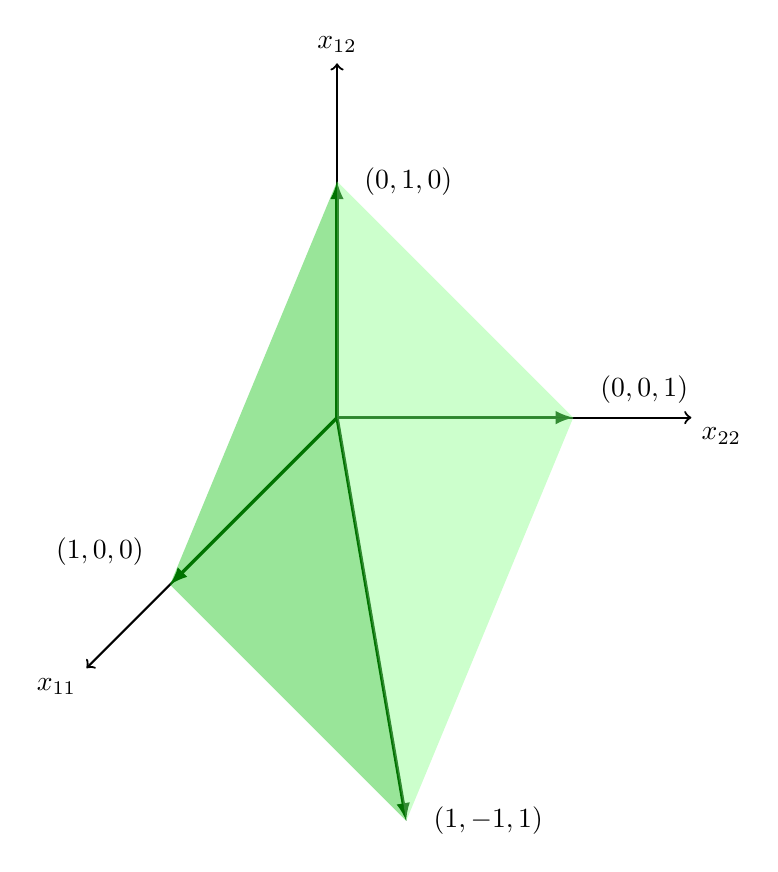
\begin{tikzpicture}%
        [x={(-0.707106cm, -0.707106cm)},
        y={(1cm, 0cm)},
        z={(0cm, 1cm)},
        scale=3.000000,
        back/.style={loosely dotted, thin},
        edge/.style={color=blue!50!black, very thick},
        facet/.style={fill=green!50!white,fill opacity=0.400000},
        facet2/.style={fill=green!75!black,fill opacity=0.400000},
        vertex/.style={inner sep=1pt,circle,draw=blue!50!black,fill=blue!50!black,thick}]

    %% Drawing the axes
    \draw[color=black,thick,->] (0,0,0) -- (1.5,0,0) node[anchor=north east]{$x_{11}$};
    \draw[color=black,thick,->] (0,0,0) -- (0,1.5,0) node[anchor=north west]{$x_{22}$};
    \draw[color=black,thick,->] (0,0,0) -- (0,0,1.5) node[anchor=south]{$x_{12}$};
    %% Rays for cone:   
    \draw[color=green!25!black,very thick,-latex] (0,0,0)--(0,0,1);
    \draw[color=green!25!black,very thick,-latex] (0,0,0)--(0,1,0);
    \draw[color=green!25!black,very thick,-latex] (0,0,0)--(1,0,0);
    \draw[color=green!25!black,very thick,-latex] (0,0,0)--(1,1,-1);
    %%
    %% Drawing the interior
    %%
    \fill[facet] (0, 0, 0) -- (0, 1, 0) -- (0, 0, 1) -- (0, 0, 0) -- cycle {};
    \fill[facet] (0,0,0) -- (1, 1, -1) -- (0, 1, 0) -- (0, 0, 0) -- cycle {};
    \fill[facet2] (0,0,0) -- (1,0,0) -- (1, 1, -1) -- (0, 0, 0) -- cycle {};
    \fill[facet2] (0, 0, 0) -- (1, 0, 0) -- (0, 0, 1) -- (0, 0, 0) -- cycle {};
    %%
    %% Drawing the vertices
    %%
    \node[label={[label distance=0.1cm]0:$(0,1,0)$}] at (0.00000, 0.00000, 1.00000)    {};
    \node[label={[label distance=0.1cm]15:$(0,0,1)$}] at (0.00000, 1.00000, 0.00000)     {};
    \node[label={[label distance=0.1cm]150:$(1,0,0)$}] at (1.00000, 0.00000, 0.00000)     {};
    \node[label={[label distance=0.1cm]0:$(1,-1,1)$}] at (1.00000, 1.00000, -1.00000)     {};
    %%
    %%
    \end{tikzpicture}
\end{tikzfigure}
\end{minipage}
\begin{minipage}[t]{0.5\linewidth}
\begin{tikzfigure}[$\cone(\mathscr B_2)$]
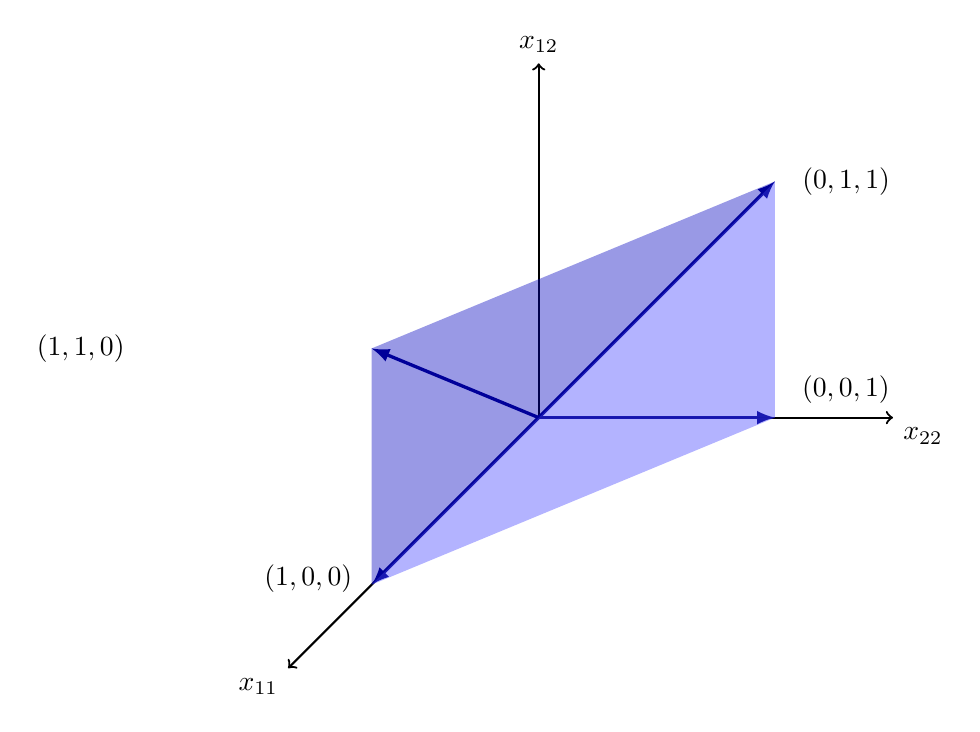
\begin{tikzpicture}%
        [x={(-0.707106cm, -0.707106cm)},
        y={(1cm, 0cm)},
        z={(0cm, 1cm)},
        scale=3.000000,
        back/.style={loosely dotted, thin},
        edge/.style={color=blue!50!black, very thick},
        facet/.style={fill=blue!75!white,fill opacity=0.400000},
        facet2/.style={fill=blue!75!black,fill opacity=0.400000},
        vertex/.style={inner sep=1pt,circle,draw=blue!50!black,fill=blue!50!black,thick}]

    %% Drawing the axes
    \draw[color=black,thick,->] (0,0,0) -- (1.5,0,0) node[anchor=north east]{$x_{11}$};
    \draw[color=black,thick,->] (0,0,0) -- (0,1.5,0) node[anchor=north west]{$x_{22}$};
    \draw[color=black,thick,->] (0,0,0) -- (0,0,1.5) node[anchor=south]{$x_{12}$};
    %% Rays for cone:   
    \draw[color=blue!50!black,very thick,-latex] (0,0,0)--(1,0,1);
    \draw[color=blue!50!black,very thick,-latex] (0,0,0)--(0,1,0);
    \draw[color=blue!50!black,very thick,-latex] (0,0,0)--(1,0,0);
    \draw[color=blue!50!black,very thick,-latex] (0,0,0)--(0,1,1);
    %%
    %% Drawing the interior
    %%
    \fill[facet] (0, 0, 0) -- (0, 1, 0) -- (0, 1, 1) -- (0, 0, 0) -- cycle {};
    \fill[facet2] (0,0,0) -- (0, 1, 1) -- (1, 0, 1) -- (0, 0, 0) -- cycle {};
    \fill[facet2] (0,0,0) -- (1,0,1) -- (1, 0, 0) -- (0, 0, 0) -- cycle {};
    \fill[facet] (0, 0, 0) -- (1, 0, 0) -- (0, 1, 0) -- (0, 0, 0) -- cycle {};
    %%
    %% Drawing the vertices
    %%
    \node[label={[label distance=0.1cm]0:$(0,1,1)$}] at (0.00000, 1.00000, 1.00000)    {};
    \node[label={[label distance=0.1cm]15:$(0,0,1)$}] at (0.00000, 1.00000, 0.00000)     {};
    \node[label={[label distance=0cm]150:$(1,0,0)$}] at (1.00000, 0.00000, -0.100000)     {};
    \node[label={[label distance=-4.5cm]0:$(1,1,0)$}] at (1.00000, 0.00000, 1.00000)     {};
    %%
    %%
    \end{tikzpicture}
\end{tikzfigure}
\end{minipage}
}
}

%\begin{comment}
%\block{4. The monomial map}{
%For $1 \leq i\leq j \leq n$, $\vect e_{ij}$ denotes a standard basis vector of $\Z^{\binom{n+1}{2}}$.
%Let 
%\begin{equation}
%\label{eq:A}
%\mathscr A_n= \{\vect e_{ij} \mid 1 \leq i \leq j \leq n\}\cup \{\vect e_{ii}-\vect e_{ij}+\vect e_{jj} \mid 1 \leq i < j \leq n\}.    
%\end{equation}
%
%We have an embedding of the torus $\Phi_{\mathscr A}: T\cong (K^*)^{\binom{n+1}{2}}\to K^{n^2}$ given by the monomial map
%\begin{equation}
%\label{eq:PhiA}
%\vect t\mapsto (t_{11},\dots,t_{nn},t_{11}t_{12}^{-1}t_{22},\dots,t_{n-1,n-1}t_{n-1,n}^{-1}t_{nn}).
%\end{equation}
%The \textbf{toric variety} is the Zariski closure of the image of $\Phi_{\mathscr A}$.
%
%\vspace{1pc}
%If we arrange the vectors in $\mathscr A$ into a matrix $A$, then the defining ideal for the toric variety can be determined using the kernel of $A$.  With $\mathscr A$ as in Equation \eqref{eq:A}, we showed that the defining ideal is exactly $\pr_2$.
%}
%\end{comment}

% % % 
\block[bodyoffsety=6.5pc, 
titleoffsety=3pc
]{4. Projective toric varieties and polytopes}{
\setlength{\columnsep}{2.35pc}
\begin{wrapfigure}{r}{0.485\linewidth}
\vspace{-20pt}
\coloredbox{
\textbf{Example.}

\vspace{1pc}
For $n=2$, $V(\pr_2)$ is %the projective variety 
$\Prj^1\times\Prj^1$ under the Segre embedding into $\Prj^3$.
\vspace{1em}
\begin{tikzfigure}[(Affine open set of) $\Prj^1\times \Prj^1\hookrightarrow \Prj^3$]
\vspace{-0.5pc}
    \begin{tikzpicture}[scale=3.5]
    \begin{scope}[scale=0.7,rotate=90, domain=-12.5:12.5,yshift=-3cm, z=(-135:sqrt(2))]
    \coordinate (p) at (0,0,0);
    \clip[above right] (-2.8,-3.2) rectangle (2.7,3);
    \draw[->,color=black] (p)--(2.3,0,0) node[left] %{\tiny $\frac{a}{b}$}
    ;
    \draw[->,color=black] (p)--(0,2.5,0) node[above] %{\tiny $\frac{au}{bv}$}
    ;
    \draw[->,color=black] (p)--(0,0,2.6) node[above right] %{\tiny $\frac{u}{v}$}
    ;
    \begin{scope}[scale=0.05,color=red!65!white]
    \def\scx{3.1}
    \def\scy{0.23}
    \foreach \u in {-12.00,-10.5,...,12.00}{
    \draw plot (\scx*\u,\scy*\x*\u,\x);
    \draw plot (\scx*\x,\scy*\u*\x,\u);
    };
    \end{scope};
    \end{scope};
\end{tikzpicture}
\end{tikzfigure}
%\vspace{1em}
}
\end{wrapfigure}%
\textbf{Projective space} $\mathbb{P}^{s-1}$ is the set of $1$-dimensional linear subspaces of $K^{s}$. We identify points in $\mathbb{P}^{s-1}$ by $[z_0:\cdots:z_{s-1}]$ where $[z_0:\cdots:z_{s-1}] = [tz_0:\cdots:tz_{s-1}]$ for all $t \in K^{\ast}$.

\vspace{1pc}
Given a homogeneous ideal $I$ contained in $K[x_0,\ldots,x_{s-1}]$, the \textbf{projective variety} is \begin{multline*}
    \mathbf{V}(I) = \{\vect [z_0 : \cdots : z_{s-1}] \in \mathbb{P}^{s-1} \\ \mid f(z_0,\ldots,z_{s-1}) = 0 \ \text{for all} \ f \in I\}.
\end{multline*}

Since $\pr_2$ is homogeneous, it defines a projective variety. Furthermore, we get a \textbf{projective toric variety} $X_{\mathscr{A}}$,
which is defined by the Zariski closure of the image of the monomial map onto projective coordinates. 

%\vspace{2pc}

\vspace{1pc}
For affine toric varieties $Y_\mathscr{A}$, we study $\cone(\mathscr{A})$. For projective toric varieties $X_{\mathscr{A}}$, we instead study the \textbf{convex hull} of $\mathscr{A}$, given by: \\$\conv(\mathscr{A}) = \left\{\sum_{\vect a\in \mathscr{A}}\lambda_{\vect a}\vect a\mid \lambda_{\vect a} \geq 0,\sum_{\vect a\in \mathscr{A}}\lambda_{\vect a} = 1\right\}.$
%The convex hull of $\mathscr{C}=\{\vect m_1,\ldots,\vect m_s\}\subset \mathbb{Z}^d$ is $\conv \mathscr{C} = \left\{\sum_{i=1}^{s} \lambda_i \vect m_i \; \middle\vert \; \lambda_i \geq 0, \; \sum_{i=1}^{s} \lambda_i = 1\right\}$.
}


% % % % % 
\column{0.33}
% % % 
\begin{subcolumns}
\subcolumn{.5}
%\vspace*{-5.25pc}
\block{}{
\vspace{-3pc}
We define the following: A \textbf{polytope} is a convex hull of a finite set of points. A \textbf{halfspace} is $H_{\vect u,b}^{+}=\{\vect x\in \R^d \mid \langle \vect x,\vect u\rangle \leq b\}$ and a \textbf{hyperplane} is $H_{\vect u,b}=\{\vect x\in \R^d \mid \langle \vect x,\vect u\rangle = b\}$ where $\vect u \in \R^d$ and $b \in \R$. A \textbf{face} $Q$ of a polytope $P$ is 
$Q = P \cap H_{\vect u, b}$ where $H_{\vect u, b}^+ \supseteq P$. \textbf{Vertices}, \textbf{edges}, and \textbf{facets} are faces of dimension $0$, $1$, and $\dim(P)-1$, respectively.

\vspace{1pc}
\innerblock{}{
\begin{thm}Let $P_n = \conv (\mathscr{A}_n)$.

The facets of $P_n$ are exactly the sets $P_n \cap H_{\vect u, 0}$ for all $\vect u \in \mathscr{B}_n$.
\end{thm}
}
}
\subcolumn{.5}
%\vspace*{-5.25pc}
\block{}{
\vspace{-3pc}
\coloredbox{
%\begin{minipage}[t]{0.5\linewidth}
\textbf{Example.}
\vspace{1pc}

%Note that $P_n = \conv(\mathscr{A}_n) \subset \R^{\binom{n+1}{2}}$ lies in the hyperplane $H_{\vect e_{11} + \vect e_{12} + \cdots + \vect e_{nn},1}$ and so $\dim P_n = \binom{n+1}{2}-1$. For example, $P_2=\conv(\mathscr{A}_2) \subset \R^3$ lies in the hyperplane $x_{11}+x_{12}+x_{22}=1$ and so $\dim P_2=2$.
%\end{minipage}
%\begin{minipage}[t]{0.5\linewidth}
%\vspace{-2pc}
\begin{tikzfigure}[$P_2 = \conv (\mathscr{A}_2)$]
%\resizebox{!}{7.5em}{
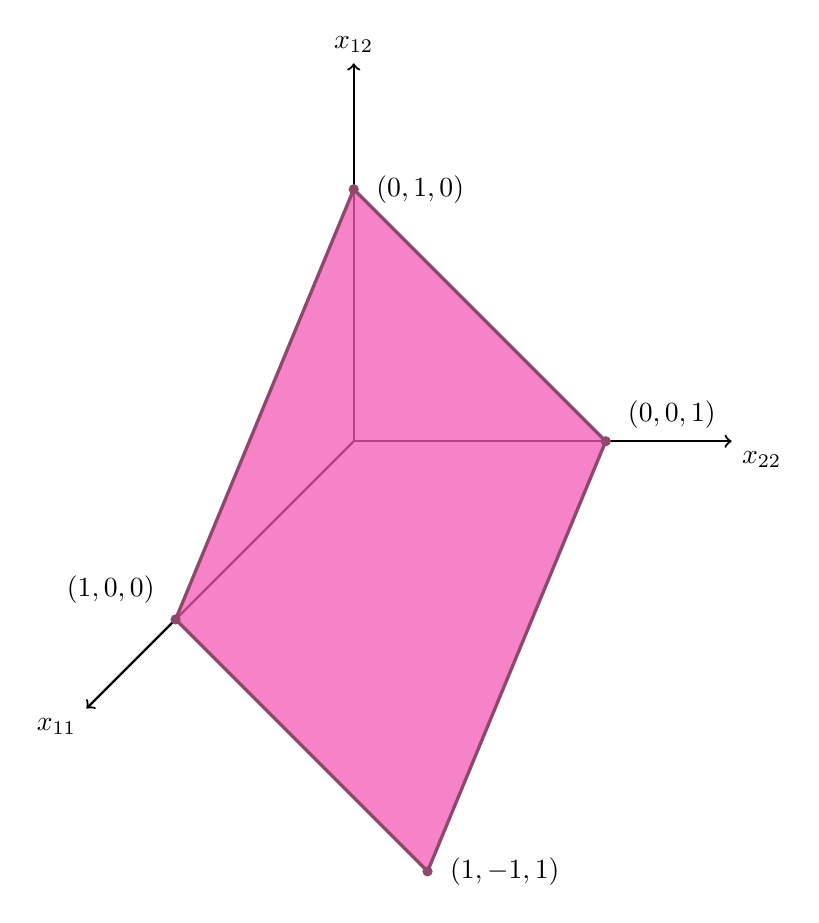
\begin{tikzpicture}%
        [x={(-0.707106cm, -0.707106cm)},
        y={(1cm, 0cm)},
        z={(0cm, 1cm)},
        scale=3.200000,
        back/.style={loosely dotted, thin},
        edge/.style={color=magenta!50!black, very thick},
        facet/.style={fill=magenta!65!white,fill opacity=0.750000},
        vertex/.style={inner sep=1pt,circle,draw=magenta!50!black,fill=magenta!50!black,thick}]
    %
    %
    %% This TikZ-picture was produced with Sagemath version 9.6
    %% with the command: ._tikz_2d_in_3d and parameters:
    %% view = [-0.124500000000000, -0.300500000000000, -0.945600000000000]
    %% angle = 145
    %% scale = 2
    %% edge_color = orange
    %% facet_color = orange
    %% opacity = 0.400000000000000
    %% vertex_color = blue
    %% axis = True
    
    %% Drawing the axes
    \draw[color=black,thick,->] (0,0,0) -- (1.5,0,0) node[anchor=north east]{$x_{11}$};
    \draw[color=black,thick,->] (0,0,0) -- (0,1.5,0) node[anchor=north west]{$x_{22}$};
    \draw[color=black,thick,->] (0,0,0) -- (0,0,1.5) node[anchor=south]{$x_{12}$};
    %% Coordinate of the vertices:
    %%
    \coordinate (0.00000, 0.00000, 1.00000) at (0.00000, 0.00000, 1.00000);
    \coordinate (0.00000, 1.00000, 0.00000) at (0.00000, 1.00000, 0.00000);
    \coordinate (1.00000, 0.00000, 0.00000) at (1.00000, 0.00000, 0.00000);
    \coordinate (1.00000, 1.00000, -1.00000) at (1.00000, 1.00000, -1.00000);
    %%
    %%
    %% Drawing the interior
    %%
    \fill[facet] (1.00000, 1.00000, -1.00000) -- (0.00000, 1.00000, 0.00000) -- (0.00000, 0.00000, 1.00000) -- (1.00000, 0.00000, 0.00000) -- cycle {};
    %%
    %%
    %% Drawing edges
    %%
    \draw[edge] (0.00000, 0.00000, 1.00000) -- (0.00000, 1.00000, 0.00000);
    \draw[edge] (0.00000, 0.00000, 1.00000) -- (1.00000, 0.00000, 0.00000);
    \draw[edge] (0.00000, 1.00000, 0.00000) -- (1.00000, 1.00000, -1.00000);
    \draw[edge] (1.00000, 0.00000, 0.00000) -- (1.00000, 1.00000, -1.00000);
    %%
    %%
    %% Drawing the vertices
    %%
    \node[vertex,label={[label distance=0.1cm]0:$(0,1,0)$}] at (0.00000, 0.00000, 1.00000)    {};
    \node[vertex,label={[label distance=0.1cm]15:$(0,0,1)$}] at (0.00000, 1.00000, 0.00000)     {};
    \node[vertex,label={[label distance=0.1cm]150:$(1,0,0)$}] at (1.00000, 0.00000, 0.00000)     {};
    \node[vertex,label={[label distance=0.1cm]0:$(1,-1,1)$}] at (1.00000, 1.00000, -1.00000)     {};
    %%
    %%
    \end{tikzpicture}
    %}
\end{tikzfigure}
\vspace{-1pc}
%\end{minipage}
}
}
\end{subcolumns}
\block{}{
\vspace{-10pc}
\innerblock{}{
\begin{thm}
\begin{enumerate}[(a)]
    \item The polytope $P_n$ is normal (i.e.,
    $kP_n \cap \mathbb{Z}^{\binom{n+1}{2}}= \sum_{i=1}^k (P_n \cap \mathbb{Z}^{\binom{n+1}{2}})$
    for all $k \geq 1$), so $X_{\mathscr{A}_n}$ is normal.
    \item When $n\geq 3$, $P_n$ is not smooth (i.e., for some vertex $v$ and all edges $E \supseteq v$, the set of generators of all $\cone(E-v)$ do not a part of a $\mathbb{Z}$-basis of $\mathbb{Z}^{\binom{n+1}{2}}$), so $X_{\mathscr{A}_n}$ is not smooth.
\end{enumerate}
\end{thm}
}
}

%\block{}{
%\vspace{-5.25pc}

%\vspace{1pc}
%A \textbf{projective variety} is a variety in projective space. The defining ideal of a projective variety is \textbf{homogeneous}, meaning its generators are polynomials with equal degree in each term.  
%Since $\pr_2$ is homogeneous, the variety $\mathbf{V}(pr_2):=\{\vect a \in \mathbb{P}^{d-1} \mid f(\vect a) = 0 \ \text{for all}\ f \in \pr_2\}$ is a projective variety.  
%\vspace{1pc}
%The projective toric variety $X_P$ is given by monomial map in Equation \eqref{eq:PhiA} with the lattice points $P\cap \Z^{\binom{n+1}{2}}=\mathscr A$, where $\mathscr A$ is as in Equation \eqref{eq:A}, and 
%\begin{equation}
%\label{eq:P}
%P = \conv(\mathscr A) = \left\{\sum_{\vect m\in\mathscr A}\lambda_{\vect m}\vect m \mid \lambda_{\vect m}\geq 0 \text{ for all }\vect m\in\mathscr A, \sum_{\vect m\in\mathscr A}\lambda_{\vect m}=1 \right\}
%\end{equation}
%is the defining polytope.
%\vspace{1pc}

%}

% % %
\block[bodyoffsety=6.5pc, 
titleoffsety=3pc
]{5. The normal fan}{
\setlength{\columnsep}{2.35pc}
\begin{wrapfigure}{r}{0.485\linewidth}
\vspace{-20pt}
\coloredbox{
\textbf{Example.}
\begin{tikzfigure}[Normal fan of $P_2$.  The intersection of the  cones is the subspace $\Span\{(1,1,1)\}$.\par]
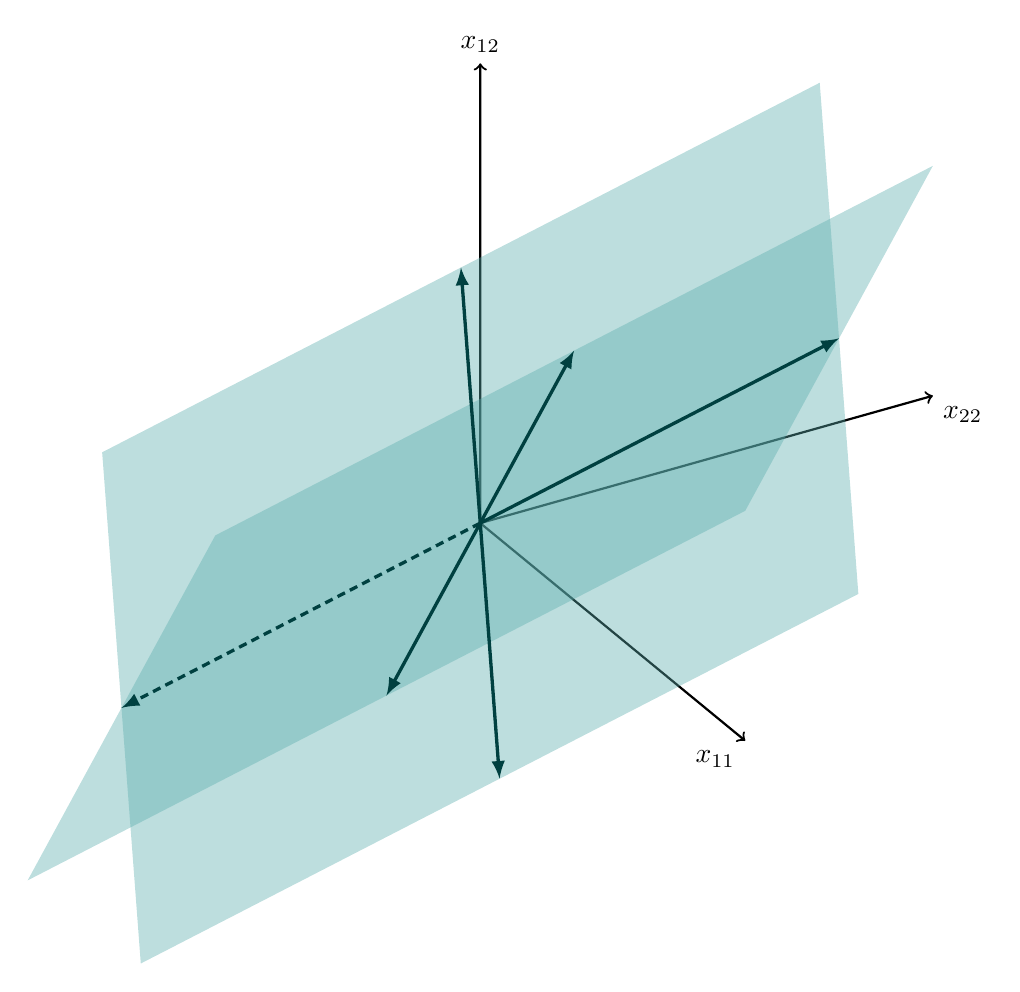
\begin{tikzpicture}%
        %[x={(0.613395cm, -0.260433cm)},
	    %y={(0.782463cm, 0.328575cm)},
	    %z={(-0.107230cm, 0.907862cm)},
        %[x={(0.800797cm, -0.258060cm)},
        %y={(0.598547cm, 0.312295cm)},
        %z={(0.021580cm, 0.914263cm)},
        [x={(0.505216cm, -0.414953cm)},
        y={(0.862993cm, 0.242833cm)},
        z={(0.000089cm, 0.876839cm)},
        scale=3.33000000,
        back/.style={loosely dotted, thin},
        edge/.style={color=teal!50!black, thick},
        facet1/.style={fill=teal!65!white,fill opacity=0.400000}]
    %
    %
    %% This TikZ-picture was produced with Sagemath version 9.6
    %% with the command: ._tikz_2d_in_3d and parameters:
    %% view = [-0.567900000000000, -0.474900000000000, -0.672300000000000]
    %% angle = 102.410000000000
    %% scale = 2
    %% edge_color = blue!50!black
    %% facet_color = blue!75!black
    %% opacity = 0.400000000000000
    %% vertex_color = black
    %% axis = True
    
    %% Drawing the axes
    \draw[color=black,thick,->] (0,0,0) -- (2,0,0) node[anchor=north east]{$x_{11}$};
    \draw[color=black,thick,->] (0,0,0) -- (0,2,0) node[anchor=north west]{$x_{22}$};
    \draw[color=black,thick,->] (0,0,0) -- (0,0,2) node[anchor=south]{$x_{12}$};
    %%
    %% Drawing the interior
    %%
    \fill[facet1] (0, 0, 0) -- (1,-0.5,-0.5) -- (0,-1.5,-1.5) -- (-1,-1,-1) -- (0, 0, 0) -- cycle {};
    \fill[facet1] (0, 0, 0) -- (1,-1,0) -- (0,-2,-1) -- (-1,-1,-1) -- (0, 0, 0) -- cycle {};
    \fill[facet1] (0, 0, 0) -- (1,-0.5,-0.5) -- (2,0.5,0.5) -- (1,1,1) -- (0, 0, 0) -- cycle {};
    \fill[facet1] (0, 0, 0) -- (1,-1,0) -- (2,0,1) -- (1,1,1) -- (0, 0, 0) -- cycle {};
    \fill[facet1] (0, 0, 0) -- (-1,0.5,0.5) -- (-2,-0.5,-0.5) -- (-1,-1,-1) -- (0, 0, 0) -- cycle {};
    \fill[facet1] (0, 0, 0) -- (-1,0.5,0.5) -- (0,1.5,1.5) -- (1,1,1) -- (0, 0, 0) -- cycle {};
    \fill[facet1] (0, 0, 0) -- (-1,1,0) -- (-2,0,-1) -- (-1,-1,-1) -- (0, 0, 0) -- cycle {};
    \fill[facet1] (0, 0, 0) -- (-1,1,0) -- (0,2,1) -- (1,1,1) -- (0, 0, 0) -- cycle {};
    
    %% Rays for normal cones:   
    \draw[color=teal!50!black,very thick,-latex] (0,0,0)--(1,-0.5,-0.5);
    \draw[color=teal!50!black,very thick,-latex] (0,0,0)--(1,-1,0);
    \draw[color=teal!50!black,very thick,-latex] (0,0,0)--(-1,1,0);
    \draw[color=teal!50!black,very thick,-latex] (0,0,0)--(-1,0.5,0.5);
    \draw[color=teal!50!black,very thick,-latex] (0,0,0)--(1,1,1);
    \draw[densely dashed, color=teal!50!black,very thick,-latex] (0,0,0)--(-1,-1,-1);
    %% Drawing the vertices
    %%
    %\node[label={[label distance=0.1cm]0:$(0,1,1)$}] at (0.00000, 1.00000, 1.00000)    {};
    %\node[label={[label distance=0.1cm]15:$(0,0,1)$}] at (0.00000, 1.00000, 0.00000)     {};
    %\node[label={[label distance=0.1cm]150:$(1,0,0)$}] at (1.00000, 0.00000, 0.00000)     {};
    %\node[label={[label distance=-2cm]0:$(1,1,0)$}] at (1.00000, 0.00000, 1.00000)     {};
    %%
    %%
    \end{tikzpicture}
\end{tikzfigure}
}
\end{wrapfigure}
Given a polytope $P$%\subset M_{\R} \cong \R^{d}$
, its  \textbf{normal fan} $\Sigma_{P}$ consists of the cones
\[
    \sigma_F = \left\{
        \vect u \in \R^d \mid F\subseteq
        \argmax_{\vect x \in P} \vect \langle \vect u, \vect x \rangle
    \right\}
\]
where $F$ is some face contained in $P$. 
%\block {}{

\vspace{1pc}
%A polytope $P$ also has a \textbf{normal fan} $\Sigma_P$, consisting of cones whose ray generators are normal to the faces of $P$.  
%\vspace{-8pc} % another janky solution
The normal fan can be obtained using information from the faces of $P$.  A projective toric variety $X_{\Sigma_P}$ can be constructed using the normal fan of $P$: the affine open subsets of $X_{\Sigma_P}$ have coordinate rings that are exactly the affine semigroup rings given by the cones in the fan. We can compute the torus orbits and the divisor class group of $X_{\Sigma_P}$ using the normal fan.%, and $X_{\Sigma_P}\cong X_P$.

%\vspace{2.5pc}
\innerblock{}{
\begin{thm} Let $\Sigma_{P_n}$ be the normal fan of $P_n$.
\begin{enumerate}[(a)]
\item The variety $X_{\mathscr{A}_n}$ is equal to $X_{\Sigma_{P_n}}$, which is normal and separated (i.e., it is Hausdorff in the classical topology).
\item Since $\Sigma_{P_n}$ is complete (i.e., $\bigcup_{\sigma \in \Sigma_{P_n}} \sigma = \R^\binom{n+1}{2}$), $X_{\mathscr{A}_n}$ is compact in both the classical and Zariski topologies.
\end{enumerate}
\end{thm}
}
}

% % % 
%\block {Further research}{
%With the normal fan of our polytope $P$, the next step in our research is to compute the divisor class group of $V(\pr_2)$.
%}

% % % 
\block[bodyoffsety=6.5pc, 
titleoffsety=3pc
]{Acknowledgements \& references}{
%\begin{spacing}{\baselinestretch}
\small
The authors thank Justin Chen, Martin Helmer, Frank Sottile, and Josephine Yu for helpful conversations.  We also thank David Cox, John Little, and Hal Schenck for their email correspondence. This project arose from the 2022 Georgia Tech REU, which is supported by 3M, NSF DMS grant \#1851843, and NSF DMS grant \#1745583.
%\end{spacing}
%}
%
% % % 
%\block[bodyoffsety=6.5pc, 
%titleoffsety=3pc
%]{References}{

\begin{biblist}

\bib{cox+little+schenck}{book}{
    AUTHOR = {Cox, David A.},
    AUTHOR = {Little, John B.},
    AUTHOR = {Schenck, Henry K.},
     TITLE = {Toric varieties},
    SERIES = {Graduate Studies in Mathematics},
    VOLUME = {124},
 PUBLISHER = {American Mathematical Society, Providence, RI},
      YEAR = {2011},
     PAGES = {xxiv+841},
      ISBN = {978-0-8218-4819-7},
   MRCLASS = {14M25 (05A15 05E45 52B12)},
  MRNUMBER = {2810322},
MRREVIEWER = {Ivan Arzhantsev},
       DOI = {10.1090/gsm/124},
       URL = {https://doi.org/10.1090/gsm/124},
}

\bib{griffin+tsatsomeros}{article}{
    AUTHOR = {Griffin, Kent},
    author = {Tsatsomeros, Michael J.},
     TITLE = {Principal minors. {II}. {T}he principal minor assignment
              problem},
   JOURNAL = {Linear Algebra Appl.},
  FJOURNAL = {Linear Algebra and its Applications},
    VOLUME = {419},
      YEAR = {2006},
    NUMBER = {1},
     PAGES = {125--171},
      ISSN = {0024-3795},
   MRCLASS = {15A29 (15A15 15A57 68Q25 90-08)},
  MRNUMBER = {2263115},
MRREVIEWER = {Udrea P\u{a}un},
       DOI = {10.1016/j.laa.2006.04.009},
       URL = {https://doi.org/10.1016/j.laa.2006.04.009},
}

\bib{wheeler}{article}{
    AUTHOR = {Wheeler, Ashley K.},
     TITLE = {Ideals generated by principal minors},
   JOURNAL = {Illinois J. Math.},
  FJOURNAL = {Illinois Journal of Mathematics},
    VOLUME = {59},
      YEAR = {2015},
    NUMBER = {3},
     PAGES = {675--689},
      ISSN = {0019-2082},
   MRCLASS = {13C40 (14M12)},
  MRNUMBER = {3554228},
MRREVIEWER = {N. Mohan Kumar},
       URL = {http://projecteuclid.org/euclid.ijm/1475266403},
}
\end{biblist}
}
\end{columns}

\end{document}